\documentclass{scrartcl}
\usepackage{graphicx,tikz}
\usepackage{siunitx}
\usepackage[graphics,tightpage,active]{preview}
\newlength\imagewidth
\newlength\imagescale
\begin{document}
%%%%%%%%%%%%%%%%%%%%%%%%%%
	\newcommand{\imsize}{.333\linewidth}
	\pgfmathsetlength{\imagewidth}{\imsize}%
	\pgfmathsetlength{\imagescale}{\imagewidth/1770}%
	\def\x{1094} % scalebar-x at golden ratio of x=1770px
	\def\y{853} % scalebar-y at 90% of height of y=948px
\begin{preview}
	%%%%%%%%%%%%%%%
	\begin{tikzpicture}[x=\imagescale,y=-\imagescale]
		\node[anchor=north west, inner sep=0pt, outer sep=0pt] at (0,0) {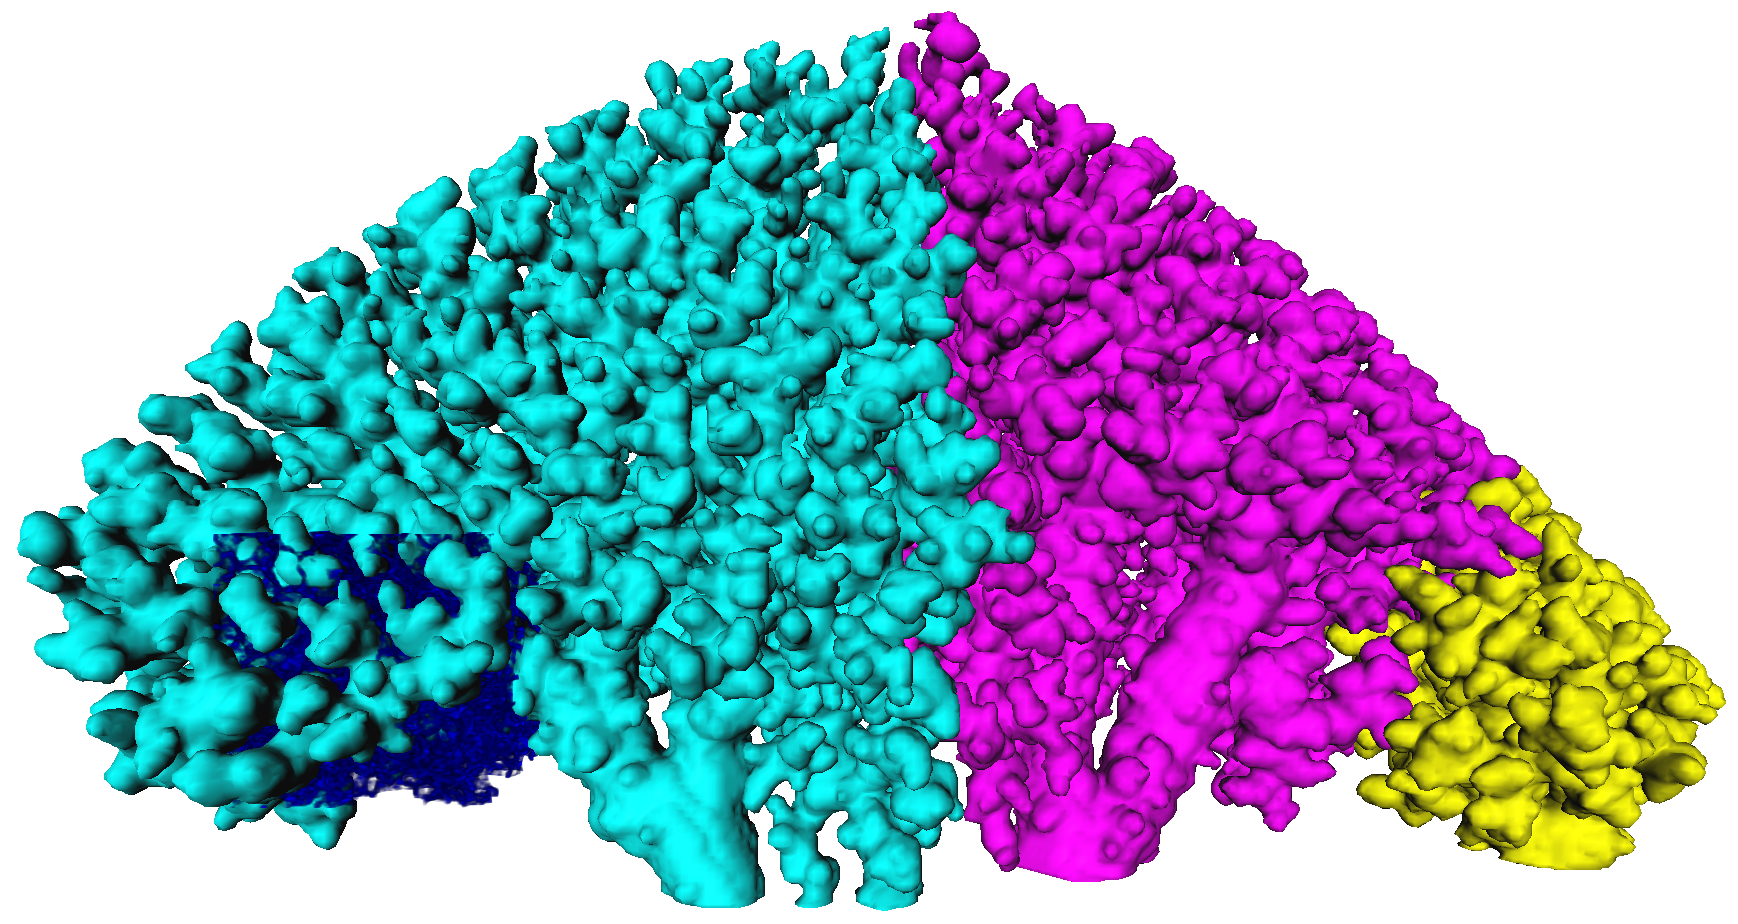
\includegraphics[width=\imagewidth]{../img/comparisonBvsT/ob}};
		% 1415px = 1.9568mm > 100px = 138um > 361px = 500um, 72px = 100um
		% \draw[|-|,thick] (340,864) -- (1747,717) node [sloped,midway,above] {\SI{1.9568}{\milli\meter} (1322.171px)};
		\draw[|-|,thick] (\x,\y) -- (\x+361,\y) node [fill=white, semitransparent, midway, above] {\SI{500}{\micro\meter}};
		\draw[|-|,thick] (\x,\y) -- (\x+361,\y) node [midway, above]{\SI{500}{\micro\meter}};
		\draw[anchor=south west] (0,948) node [fill=white, semitransparent] {(a): B} node {(a): B};
	\end{tikzpicture}%
	%%%%%%%%%%%%%%%
	\begin{tikzpicture}[x=\imagescale,y=-\imagescale]
		\node[anchor=north west, inner sep=0pt, outer sep=0pt] at (0,0) {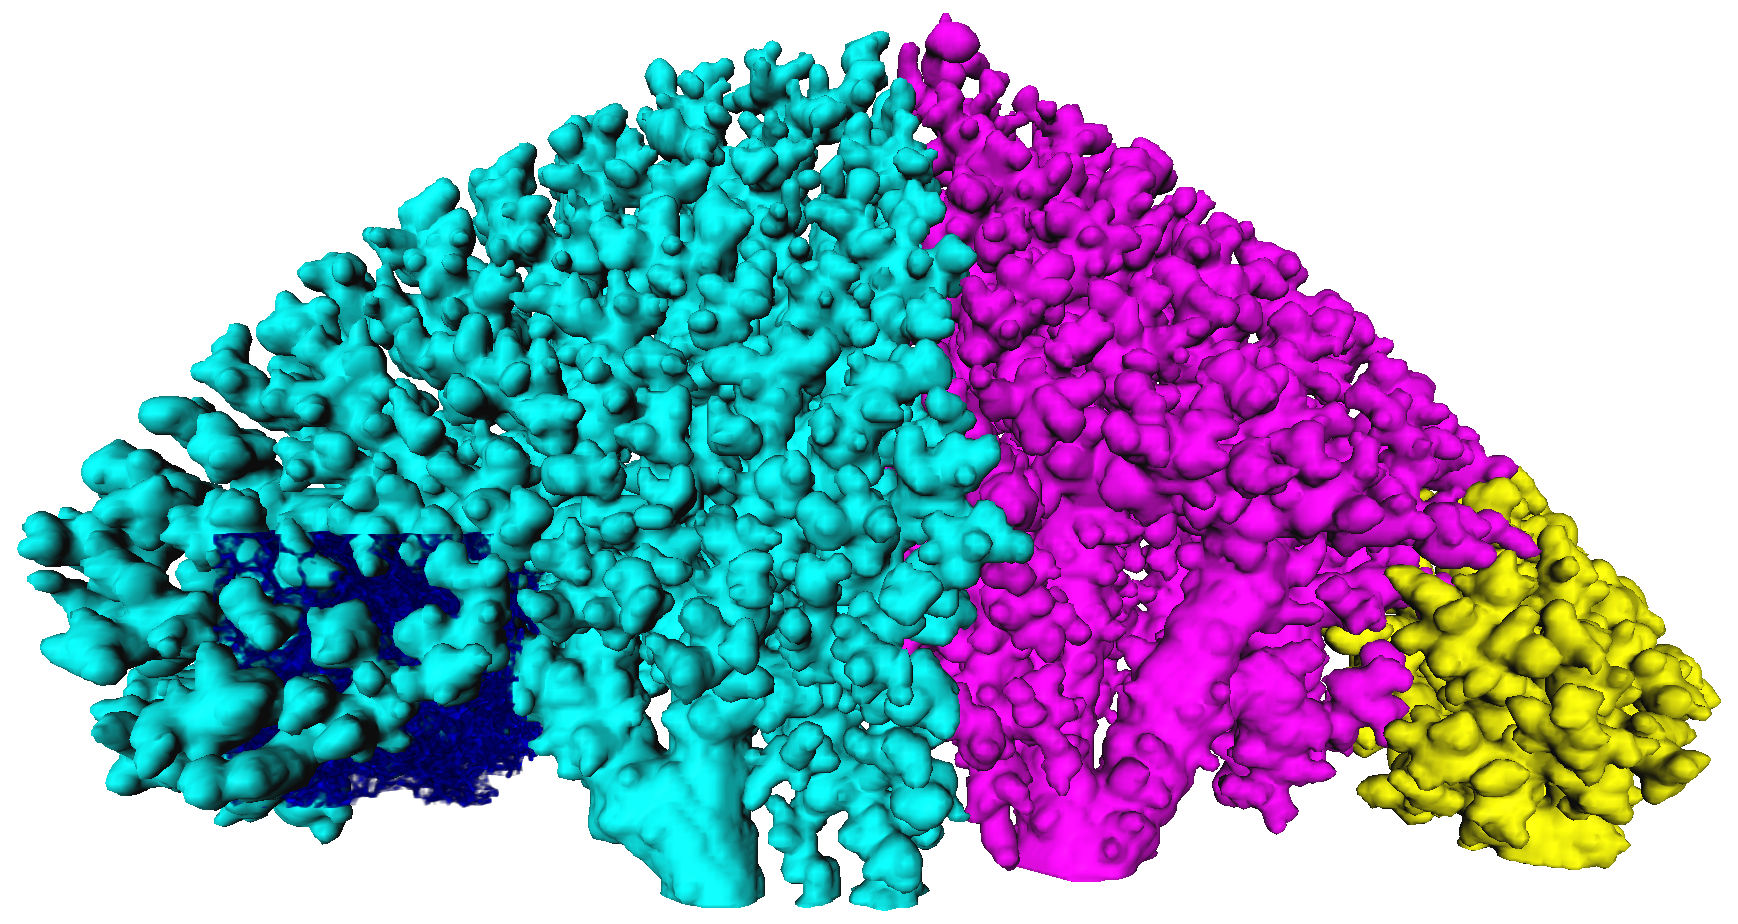
\includegraphics[width=\imagewidth]{../img/comparisonBvsT/ol}};
		% 1415px = 1.9568mm > 100px = 138um > 361px = 500um, 72px = 100um
		% \draw[|-|,thick] (340,864) -- (1747,717) node [sloped,midway,above] {\SI{1.9568}{\milli\meter} (1322.171px)};
		\draw[|-|,thick] (\x,\y) -- (\x+361,\y) node [fill=white, semitransparent, midway, above] {\SI{500}{\micro\meter}};
		\draw[|-|,thick] (\x,\y) -- (\x+361,\y) node [midway, above]{\SI{500}{\micro\meter}};
		\draw[anchor=south west] (0,948) node [fill=white, semitransparent] {(b): L} node {(b): L};
	\end{tikzpicture}%
	%%%%%%%%%%%%%%%
	\begin{tikzpicture}[x=\imagescale,y=-\imagescale]
		\node[anchor=north west, inner sep=0pt, outer sep=0pt] at (0,0) {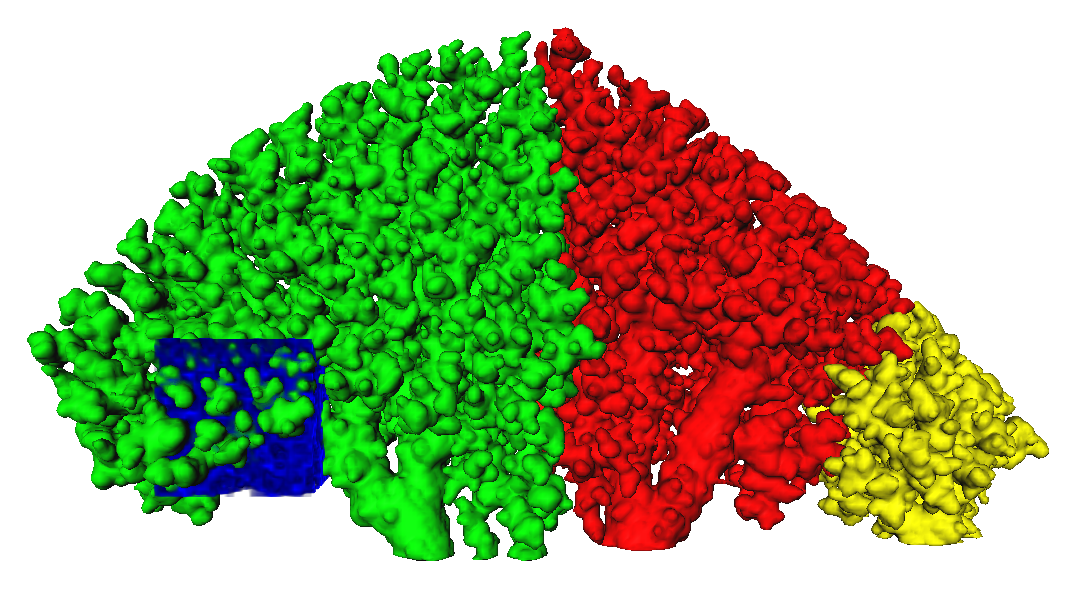
\includegraphics[width=\imagewidth]{../img/comparisonBvsT/ot}};
		% 1415px = 1.9568mm > 100px = 138um > 361px = 500um, 72px = 100um
		% \draw[|-|,thick] (340,864) -- (1747,717) node [sloped,midway,above] {\SI{1.9568}{\milli\meter} (1322.171px)};
		\draw[|-|,thick] (\x,\y) -- (\x+361,\y) node [fill=white, semitransparent, midway, above] {\SI{500}{\micro\meter}};
		\draw[|-|,thick] (\x,\y) -- (\x+361,\y) node [midway, above]{\SI{500}{\micro\meter}};
		\draw[anchor=south west] (0,948) node [fill=white, semitransparent] {(c): T} node {(c): T};
	\end{tikzpicture}%
	%%%%%%%%%%%%%%%
	\pgfmathsetlength{\imagewidth}{\imsize}%
	\pgfmathsetlength{\imagescale}{\imagewidth/799}%
	\def\x{494} % scalebar-x at golden ratio of x=799px
	\def\y{720} % scalebar-y at 90% of height of y=800px
	%%%%%%%%%%%%%%%
	\begin{tikzpicture}[x=\imagescale,y=-\imagescale]
		\node[anchor=north west, inner sep=0pt, outer sep=0pt] at (0,0) {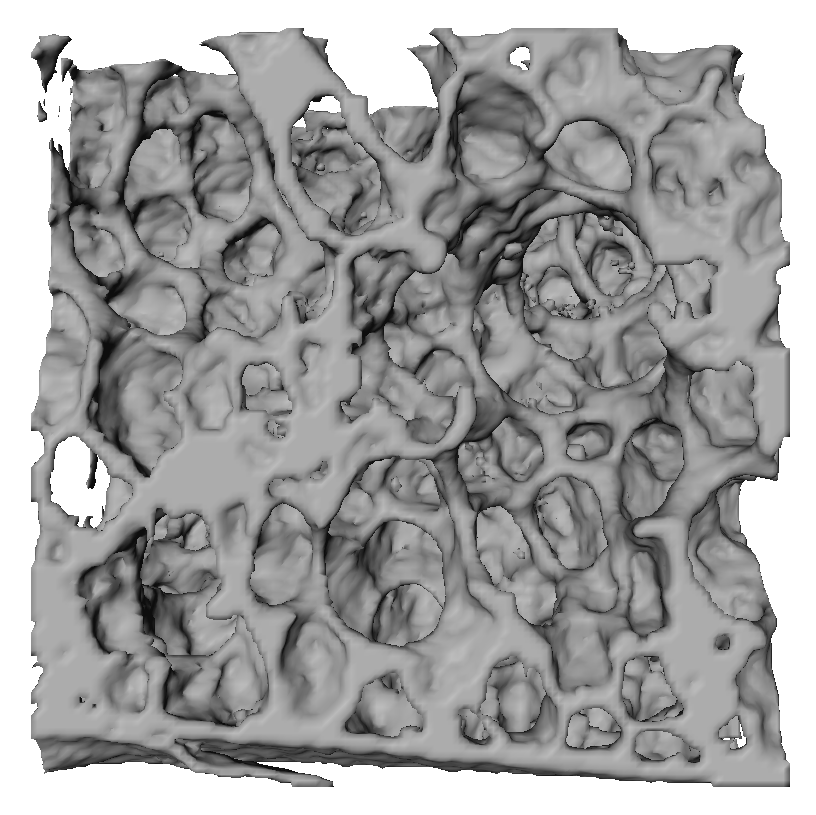
\includegraphics[width=\imagewidth]{../img/comparisonBvsT/roiB}};
		% 758px = 0.37888mm > 100px = 50um > 1000px = 500um, 200px = 100um
		% \draw[|-|,thick] (20,138) -- (778,136) node [sloped,midway,above] {\SI{0.37888}{\milli\meter} (256px)};
		\draw[|-|,thick] (\x,\y) -- (\x+100,\y) node [fill=white, semitransparent, midway, above] {\SI{50}{\micro\meter}};
		\draw[|-|,thick] (\x,\y) -- (\x+100,\y) node [midway, above]{\SI{50}{\micro\meter}};
		\draw[anchor=south west] (0,800) node [fill=white, semitransparent] {(d): B} node {(d): B};
	\end{tikzpicture}%
	%%%%%%%%%%%%%%%
	\begin{tikzpicture}[x=\imagescale,y=-\imagescale]
		\node[anchor=north west, inner sep=0pt, outer sep=0pt] at (0,0) {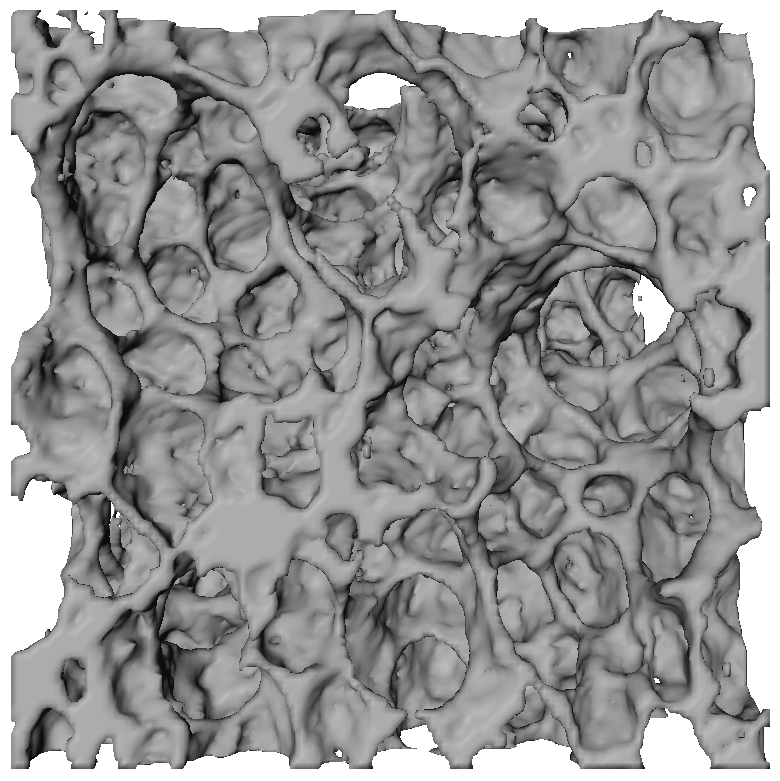
\includegraphics[width=\imagewidth]{../img/comparisonBvsT/roiL}};
		% 758px = 0.37888mm > 100px = 50um > 1000px = 500um, 200px = 100um
		% \draw[|-|,thick] (20,138) -- (778,136) node [sloped,midway,above] {\SI{0.37888}{\milli\meter} (256px)};
		\draw[|-|,thick] (\x,\y) -- (\x+100,\y) node [fill=white, semitransparent, midway, above] {\SI{50}{\micro\meter}};
		\draw[|-|,thick] (\x,\y) -- (\x+100,\y) node [midway, above]{\SI{50}{\micro\meter}};
		\draw[anchor=south west] (0,800) node [fill=white, semitransparent] {(e): L} node {(e): L};
	\end{tikzpicture}%
	%%%%%%%%%%%%%%%
	\begin{tikzpicture}[x=\imagescale,y=-\imagescale]
		\node[anchor=north west, inner sep=0pt, outer sep=0pt] at (0,0) {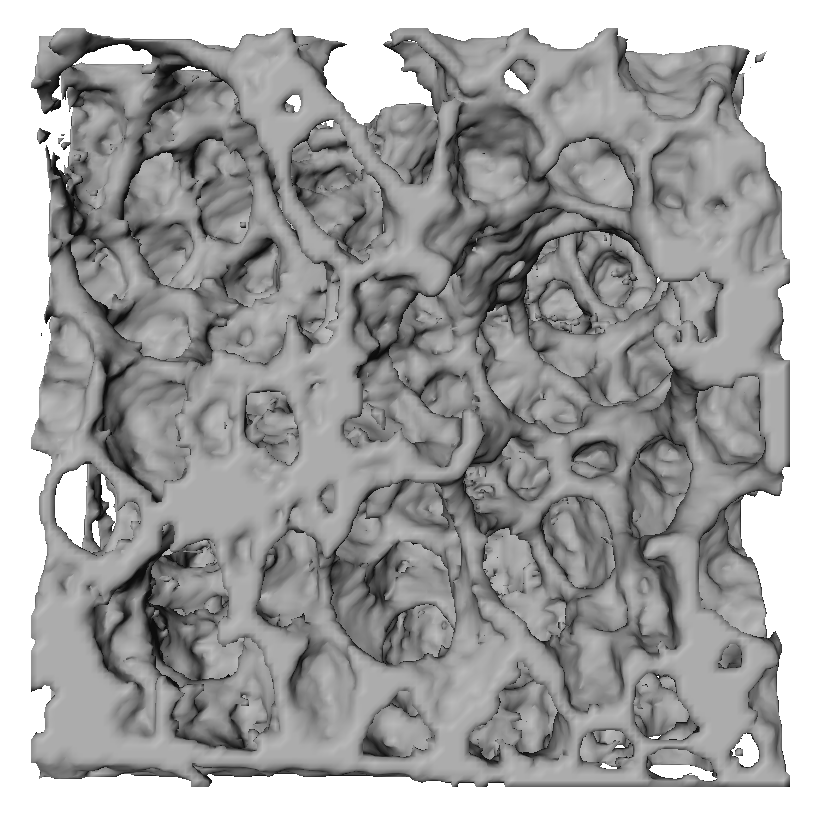
\includegraphics[width=\imagewidth]{../img/comparisonBvsT/roiT}};
		% 758px = 0.37888mm > 100px = 50um > 1000px = 500um, 200px = 100um
		% \draw[|-|,thick] (20,138) -- (778,136) node [sloped,midway,above] {\SI{0.37888}{\milli\meter} (256px)};
		\draw[|-|,thick] (\x,\y) -- (\x+100,\y) node [fill=white, semitransparent, midway, above] {\SI{50}{\micro\meter}};
		\draw[|-|,thick] (\x,\y) -- (\x+100,\y) node [midway, above]{\SI{50}{\micro\meter}};
		\draw[anchor=south west] (0,800) node [fill=white, semitransparent] {(f): T} node {(f): T};
	\end{tikzpicture}%
	%%%%%%%%%%%%%%%
\end{preview}
%%%%%%%%%%%%%%%%%%%%%%%%%%
\end{document}